\documentclass{beamer}
\usepackage[ngerman]{babel}
\usepackage[utf8]{inputenc}
\usepackage{amsmath}
\usepackage{amsthm}
\usepackage{siunitx}
\usepackage{graphicx}
\usepackage{pgfplots}
\sisetup{locale = DE,
per-mode = fraction}
% Lade Beamer Stile
\usepackage{beamerthemesplit}
\usepackage{tcolorbox}
\usetheme{Rochester}
\usecolortheme{crane}
\usepackage{wrapfig}
\newcolumntype{C}[1]{>{\centering\arraybackslash}p{#1}@{}}

\title{4. Unterrichtseinheit zur Wärmelehre}
\subtitle{Wärmeübertragung}
\author{Heiko Schröter}
\date{\today}
\titlegraphic{
\includegraphics[scale=0.6]{logo_RHS.pdf}}
\setbeamertemplate{enumerate item}{\alph{enumi})}

\begin{document}

\frame{\titlepage}

\frame
{
  \frametitle{Ziele für die heutige Unterrichtseinheit}
  \textbf{Welche Arten der Wärmeausbreitung gibt es?}
  \begin{itemize}
	\item Wie berechnet sich der Wärmestrom bei Wärmeleitung?
	\item Wie berechnet sich der Wärmestrom bei Konvektion?
	\item Wie berechnet sich der Wärmestrom bei Wärmedurchgang durch eine Wand?
	\item Welcher Zusammenhang besteht zwischen Emission und Absorption?
	\item Wodurch sind technische Wärmeübertragungen gekennzeichnet?
  \end{itemize}
}

\frame[allowframebreaks]
{
  \frametitle{Wärmeübertragung}
  \begin{block}{Zweiter Hauptsatz und Wärmetransport}
  Bei einem Temperaturgefälle $T_1>T_2$ fließt Wärmeenergie selbsttätig vom Ort der hohen Temperatur $T_1$ zum Ort der tieferen Temperatur $T_1$.
  \end{block}
  \begin{tikzpicture}
  \begin{scope}[scale=0.05]
    \filldraw [color=red, fill=orange, very thick] (0,0) -- (50,0) -- (50,50) -- (0,50) -- cycle;
    \filldraw [color=black, fill=lightgray, very thick] (150,0) -- (200,0) -- (200,50) -- (150,50) -- cycle;
    \draw [->, >=latex, ultra thick, red] (50,25) -- (150,25) node [midway, above] {$Q$};
	\node (T1) at (25,25) {$T_1$};
	\node (T2) at (175,25) {$T_2$};
    \filldraw [color=black, fill=white, very thick] (70,-25) -- (130,-25) -- (130,5) -- (70,5) -- cycle;
    \node (T) at (100,-10) {$T_1>T_2$};	
  \end{scope}
  \end{tikzpicture}
  
\begin{block}{Wärmestrom}
Die pro Zeiteinheit $t$ in Richtung Temperaturgefälle transportierte Wärmeenergie $Q$ ist der Wärmestrom $\dot{Q}$
\begin{align*}
\dot{Q}=\dfrac{Q}{t};\quad [\dot{Q}]=\SI{1}{\joule\per\second}=\SI{1}{\watt}
\end{align*}
\end{block}
Die Übertragung von Wärmeenergie kann auf dreierlei verschiedene Arten von einem Körper auf den anderen erfolgen:
  \begin{block}{\textbf{Wärmeleitung} $\rightarrow$}
  Übertragung von Wärmeenergie zwischen direkt benachbarten Teilchen.
  \end{block}
  \begin{block}{\textbf{Wärmestrahlung} $\rightarrow$}
  Übertragung der Energie durch \textbf{Quanten} bzw. \textbf{Photonen}. Dabei ist kein Übertragungsmedium erforderlich, so z.B. von der Sonne durch das luftleere Weltall zur Erde. 
  \end{block}
  \begin{block}{\textbf{Wärmemitführung} $\rightarrow$}
  Übertragung durch einen \textbf{Wärmeträger}. Dies nennt man auch eine \textbf{Konvektion} oder \textbf{Wärmeströmung}. Man unterscheidet die \textbf{freie Konvektion} von der \textbf{erzwungenen Konvektion}.
  \end{block}
}

\frame
{
  \frametitle{Wärmeleitung}
  \begin{block}{}
  Bei der Wärmeleitung wird die Wärme innerhalb eines festen Körpers oder zwischen Körpern übertragen, die sich berühren.
  \end{block}
  \begin{figure}
	\includegraphics[width=.45\linewidth]{Wärmeleitung_1}
	\caption{Wärmeleitung in einem Metallstab}
\end{figure}
}

\frame
{
  \frametitle{Wärmeleitfähigkeit}
  \begin{block}{}
  Die Wärmeleitfähigkeit ist abhängig vom Material aus dem der Körper besteht.
  \end{block}
  \begin{figure}
	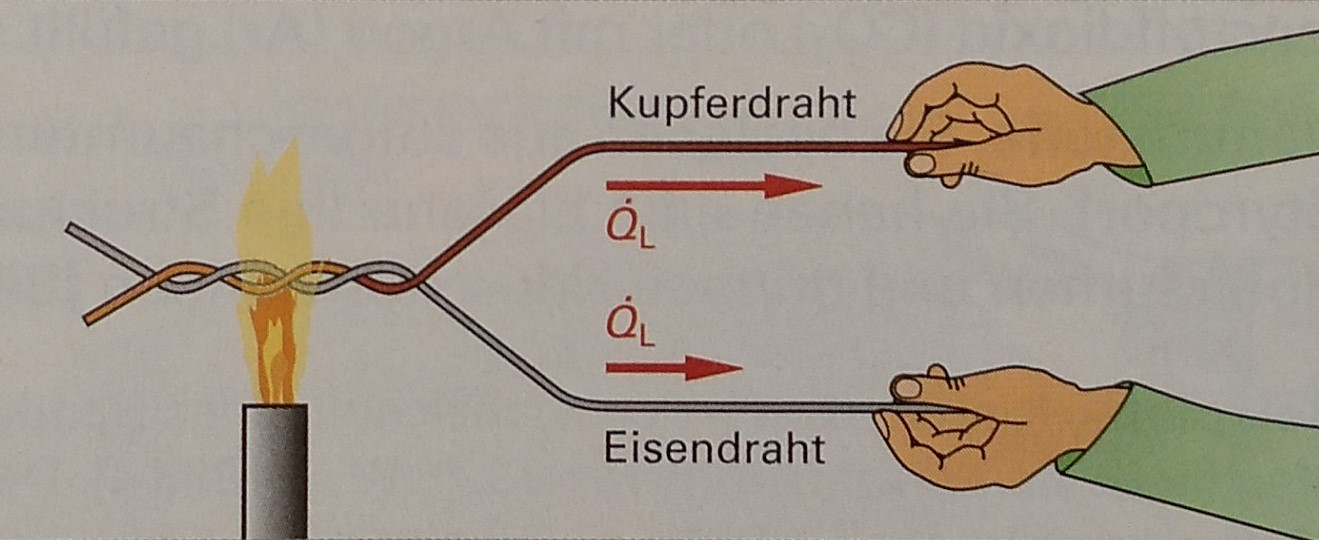
\includegraphics[width=.45\linewidth]{Wärmeleitfähigkeit}
	\caption{Wärmeleitung in einem Metallstab}
\end{figure}
}

\frame[allowframebreaks]
{
  \frametitle{Wärmestrom bei Wärmeleitung}
  \begin{block}{}
  Der Wärmestrom $\dot{Q}_L$ ist eine Leistung (Energie pro Zeit) mit der Einheit Watt bzw. Kilowatt.
  \end{block}
  Der durch einen Stab geleitete Wärmestrom ist von folgenden Größen abhängig:
\begin{itemize}
\item der Querschnittsfläche $A$ des Stabes $\Rightarrow \dot{Q}_L\sim A$
\item der Länge $l$ des Stabes $\Rightarrow \dot{Q}_L\sim \frac{1}{l}$
\item der Temperaturdifferenz $\Delta\vartheta$ zwischen den Stabenden $\Rightarrow \dot{Q}_L\sim \Delta\vartheta$
\end{itemize}

Daraus ergibt sich folgender Zusammenhang:
\begin{block}{Wärmestrom bei Wärmeleitung}
$\dot{Q}_L=\dfrac{\lambda}{l}\cdot A\cdot\Delta\vartheta\quad\quad\dot{Q}_L=\dfrac{Q_L}{t}$
  \end{block}
Die SI-Einheit der Wärmeleitfähigkeit $\lambda$ ist: 
	\begin{tcolorbox}	  
	  $\frac{W\cdot m}{m^{2}\cdot K}=\frac{W}{m\cdot K}$
	\end{tcolorbox}
Die Wärmeleitfähigkeit $\lambda$ eines Werkstoffes gibt die Wärme in Joule an, die bei einem Temperaturunterschied von \SI{1}{\kelvin} durch einen Querschnitt von \SI{1}{\square\meter} bei \SI{1}{\meter} Länge in \SI{1}{\second} hindurchtritt.
}

\frame
{
\frametitle{Beispielaufgabe Wärmestrom bei Wärmeleitung}
Durch eine Stahlplatte mit der Fläche $A=\SI{5}{\square\meter}$ und der Dicke $l=\SI{12}{\milli\meter}$ fließt eine Wärmemenge $Q=\SI{80}{\kilo\joule}$. Die Wandtemperaturen betragen $\vartheta_{1}=\SI{80}{\celsius}$ und $\vartheta_{2}=\SI{78}{\celsius}$. Berechnen Sie bei $\lambda=\SI{58}{\watt\per\meter\per\kelvin}$ die Zeit $t$ für die Wärmeübertragung.\\
\textbf{Lösung:}
\begin{align*}
Q_L&=\dfrac{\lambda}{l}\cdot A\cdot\Delta\vartheta\cdot t\\
\rightarrow t&=\dfrac{Q_L\cdot l}{\lambda\cdot A\cdot\Delta\vartheta}=\dfrac{\SI{80}{\kilo\joule}\cdot\SI{12}{\milli\meter}}{\SI{58}{\watt\per\meter\per\kelvin}\cdot \SI{5}{\square\meter}\cdot\SI{2}{\kelvin}}=\SI{1,66}{\second}
\end{align*}
}

\frame[allowframebreaks]
{
  \frametitle{Konvektion}
  \begin{block}{}
  Bei der Konvektion, auch Wärmeströmung genannt, wird die Wärme durch ein strömendes gasförmiges oder flüssiges Übertragungsmittel transportiert. Der bei der Konvektion übertragene Wärmestrom $\dot{Q}_K$ berechnet sich aus der abgegebenen Wärmemenge des strömenden Übertragungsmittels nach folgender Gleichung.
  \end{block}
\begin{block}{Wärmestrom bei Konvektion}
$\dot{Q}_K=\dot{m}\cdot c\cdot\Delta\vartheta;\quad\dot{Q}_K=\dfrac{Q_K}{t};\quad\dot{m}=\dfrac{m}{t}$
  \end{block}
\newpage
\begin{itemize}
\item freie Konvektion $\Rightarrow$ die Strömungsbewegung entsteht von selbst
\item erzwungene Konvektion $\Rightarrow$ die Strömungsbewegung wird durch umpumpen verstärkt
\end{itemize}
  \begin{figure}
	\includegraphics[width=.45\linewidth]{konvektion_f}
	\caption{freie Konvektion durch Erwärmung bzw. Abkühlung}
  \end{figure}
  \begin{figure}
	\includegraphics[width=.75\linewidth]{konvektion_e}
	\caption{Warmwasser-Zentralheizung}
  \end{figure}
}

\frame[allowframebreaks]
{
  \frametitle{Wärmedurchgang durch eine Wand}
  \begin{block}{}
Der Wärmedurchgang durch eine Wand besteht aus mindestens zwei Wärmeübergängen und einer Wärmeleitung.
  \end{block}
In technischen Geräten und Apparaten wird die Wärme häufig durch eine Wand hindurch von einem Fluid auf ein anderes Fluid übertragen.
\begin{block}{Wärmestrom bei Wärmedurchgang}
$\dot{Q}_D=k\cdot A\cdot(\vartheta_1-\vartheta_2);\quad\dot{Q}_D=\dfrac{Q_K}{t}$
  \end{block}
k ist die Wärmedurchgangszahl. Die SI-Einheit der Wärmedurchgangszahl $k$ ist: 
	\begin{tcolorbox}	  
	  $\frac{W}{m^{2}\cdot K} \Rightarrow 0.278\cdot\frac{W}{m^{2}\cdot K}=\frac{kJ}{m^{2}\cdot h\cdot K}$
	\end{tcolorbox}
Die Wärmedurchgangszahl $k$ gibt die Wärmeenergie in \si{\kilo\joule} an, die pro \si{\square\meter} Austauschfläche und Stunde bei einer Temperaturdifferenz von \SI{1}{\kelvin} übertragen wird.  
  \begin{figure}
	\includegraphics[width=.7\linewidth]{Wärmedurchgang}
	\caption{Vorgänge beim Wärmedurchgang}
  \end{figure}
}

\frame[allowframebreaks]
{
\frametitle{Beispielaufgabe Wärmedurchgang durch eine Wand}
In einem Rohrbündel-Wärmetauscher mit einer Wärmeaustauschfläche $A$ von $\SI{2,20}{\square\meter}$ wird ein Wärmestrom von $\SI{26400}{\kilo\joule\per\hour}$ übertragen. Die Temperaturdifferenz der beiden Fluide beträgt $\SI{60}{\kelvin}$. Wie groß ist die Wärmedurchgangszahl $k$?\\
  \begin{figure}
	\includegraphics[width=.75\linewidth]{Wärmetauscher}
	\caption{Rohrbündel-Wärmetauscher}
  \end{figure}
\textbf{Lösung:}
\begin{align*}
\dot{Q}_D&=k\cdot A\cdot(\vartheta_1-\vartheta_2)\\
\Rightarrow k&=\dfrac{\dot{Q}_D}{A\cdot(\vartheta_1-\vartheta_2)}=\dfrac{\SI{26400}{\kilo\joule\per\hour}}{\SI{2,20}{\square\meter}\cdot\SI{60}{\kelvin}}\\
k&=\SI{200}{\kilo\joule\per\square\meter\per\hour\per\kelvin}=200\cdot \dfrac{1000}{\SI{3600}{\per\hour}}\cdot\si{\kilo\joule\per\square\meter\per\hour\per\kelvin}=200\cdot 0.278\cdot\si{\watt\per\square\meter\per\kelvin}\\
&=\SI{55,6}{\watt\per\square\meter\per\kelvin}
\end{align*}
}

\frame[allowframebreaks]
{
  \frametitle{Emission und Absorption}
  \begin{figure}
	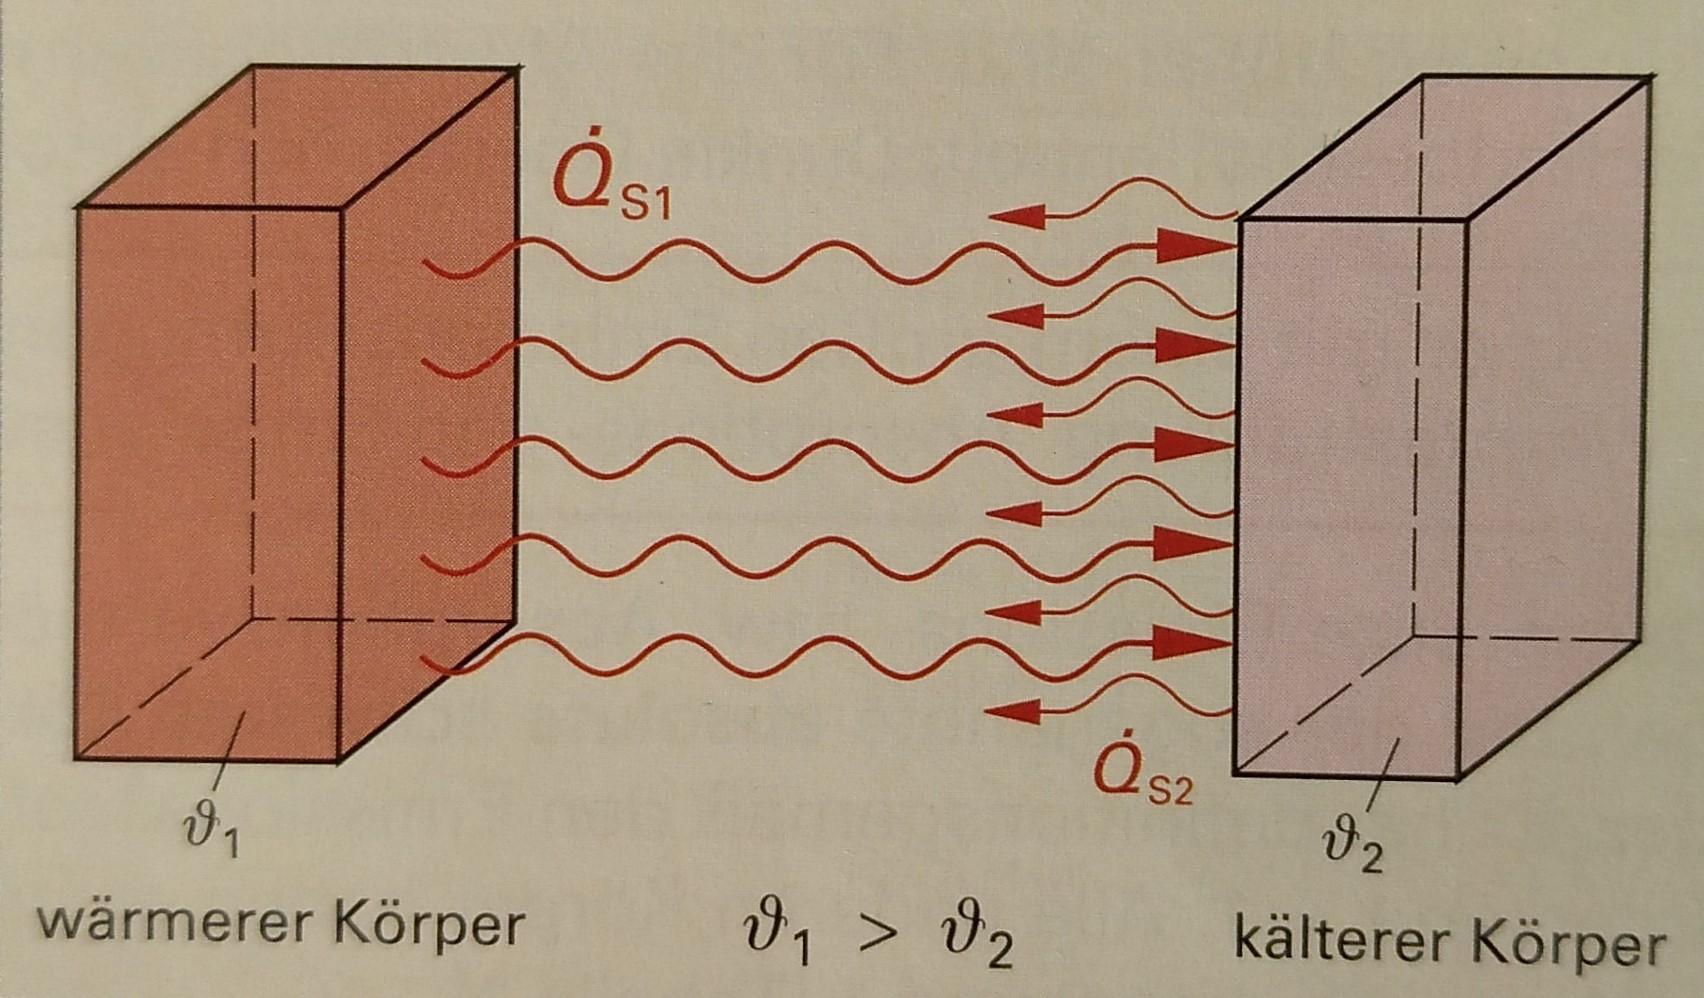
\includegraphics[width=.7\linewidth]{Strahlung}
	\caption{Abgegebene und aufgenommene Strahlung}
  \end{figure}
Jeder Körper gibt Wärmestrahlung in Form elektromagnetischer Wellen ab. Sie durchstrahlen den freien Raum und benötigen zu ihrem Transport kein Übertragungsmittel. Trifft die Strahlung auf einen Körper, so wird ein Teil der Strahlung aufgenommen (absorbiert), der andere Teil wird entweder zurückgeworfen (reflektiert) oder durchdringt den Körper.
  \begin{block}{}
Körper mit großen Emissionsvermögen haben auch ein großes Absorptionsvermögen für Wärmestrahlung. Absorptions- und Emissionsvermögen eines Körpers sind gleich groß. 
  \end{block}
\newpage
  Die von einem Körper abgegebene Wärmestrahlung ist von folgenden Größen abhängig:
\begin{itemize}
\item der Temperatur $T$ des Körpers $\Rightarrow \dot{Q}_S\sim T^{4}$
\item der Fläche $A$ $\Rightarrow \dot{Q}_S\sim A$
\item der Oberflächenbeschaffenheit ausgedrückt durch die Emissions-Konstante $\varepsilon\Rightarrow \dot{Q}_s\sim \varepsilon$
\item der Stefan-Boltzmann\footnote{Josef Stefan, österreichischer Physiker (1835 bis 1893); Ludwig Boltzmann, österreichischer Physiker (1844 bis 1906)}  Konstante $\sigma\Rightarrow \dot{Q}_s\sim \sigma$
\end{itemize}
\begin{block}{Stefan-Boltzmann'sches Gesetz}
$\dot{Q}_S=\sigma\cdot\varepsilon\cdot A\cdot T^{4}$\\
$\dot{Q}_S=C_S\cdot\varepsilon\cdot A\cdot \left(\dfrac{T}{100}\right)^{4}$
  \end{block}
Der Wert der Stefan-Boltzmann-Konstante $\sigma$ beträgt $5,67\cdot 10^{-8}\si{\watt\per\square\meter\per\kelvin\tothe{4}}$. In der Technik wird die Strahlungskonstante $C_S=\SI{5,67}{\watt\per\square\meter\per\kelvin\tothe{4}}$ verwendet. Der Faktor $10^{-8}=\left(10^{-2}\right)^{4}=\left(\frac{1}{100}\right)^{4}$ wird dann zusammen mit der Temperatur $T$ als Quotient $\left(\dfrac{T}{100}\right)^{4}$ in der Gleichung geschrieben.

}
\end{document}
